\Tekst{
Vanjska sila iznosa $F_0=42\ N$ djeluje pod kutem od $\vartheta = 30^\circ$ prema horizontali na blok $A$ mase $m_A=5 \ kg$ koji gura blok 
$B$ mase $m_B=2\ kg$ (vidjeti skicu). Izračunajte iznos ubrzanja blokova A i B kada je kinetičko trenje između blokova i podloge $\mu _k=0,3$.

\begin{figure}[h]%{r}{0.7\textwidth} % Inline image example
  \begin{center}
    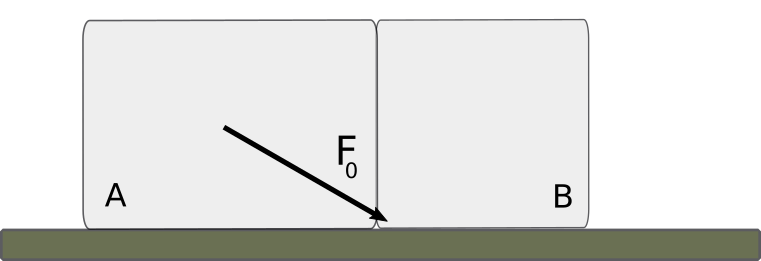
\includegraphics[scale=0.30]{../03_Dinamika_materijalne_tocke/Zadatak_D315.png}
  \end{center}
  %\caption{Fish}
\end{figure}
}
